\documentclass[usenames,dvipsnames]{beamer}

\usefonttheme{serif}
\setbeamertemplate{items}[circle]

\usepackage{pxfonts}
\usepackage{mathpazo}
\usepackage{tcolorbox}
\usepackage{soul}


% \definecolor{red}{rgb}{1,0,0}

\beamertemplatenavigationsymbolsempty

\DeclareMathOperator*{\minimize}{minimize}
\DeclareMathOperator*{\Exp}{\mathbf{E}}
\DeclareMathOperator{\Regret}{Regret}
\DeclareMathOperator{\Risk}{Risk}
\DeclareMathOperator{\polylog}{polylog}
\DeclareMathOperator*{\argmin}{argmin}
\DeclareMathOperator*{\argmax}{argmax}
\newcommand{\R}{\mathbb{R}}
\newcommand{\indicator}{\mathbf{1}}
\newcommand{\norm}[1]{\left\|#1\right\|}
\newcommand{\KL}[2]{D\left({#1}\middle\|{#2}\right)}

\newcommand{\Cite}[1]{{\tiny \textcolor{Blue}{[#1]}}}

\makeatletter
\newcommand\SoulColor{%

\let\set@color\beamerorig@set@color
\let\reset@color\beamerorig@reset@color}
\makeatother
\setstcolor{red}



\title{AdaGrad has regret larger than $T$}

\date{June 26, 2016 \\ \tiny COLT 2016}
\author{Francesco Orabona \and \underline{\textbf{D\'avid P\'al}}}
\institute{Yahoo Research, New York}

\begin{document}

%%%%%%%%%%%%%%%%%%%%%%%%%%%%%%%%%%%%%%%%%%%%%%%%%%%%%%%%%%%%%%%%%%%%%%%%%%%%%%%%%%%%%%%%%%
\begin{frame}
\maketitle
\end{frame}

%%%%%%%%%%%%%%%%%%%%%%%%%%%%%%%%%%%%%%%%%%%%%%%%%%%%%%%%%%%%%%%%%%%%%%%%%%%%%%%%%%%%%%%%%%
\begin{frame}
\frametitle{Online Linear Optimization}

Given convex set $K \subseteq \R^N$

\vspace{0.3cm}

For $t=1,2,\dots$
\begin{itemize}
\item predict $w_t \in K$
\item receive loss vector function $\ell_t \in \R^N$
\item suffer loss $\langle \ell_t, w_t \rangle$
\end{itemize}

\vspace{0.3cm}
$$
\Regret_T(u) = \textcolor{ForestGreen}{\underbrace{\sum_{t=1}^T \langle \ell_t, w_t \rangle}_{\text{algorithm's loss}}} \ - \ \textcolor{red}{\underbrace{\sum_{t=1}^T \langle \ell_t, u \rangle}_{\text{competitor's loss}}}
$$

\vspace{0.3cm}

We consider the \textbf{unbounded} domain $K = \R^N$
\end{frame}

%%%%%%%%%%%%%%%%%%%%%%%%%%%%%%%%%%%%%%%%%%%%%%%%%%%%%%%%%%%%%%%%%%%%%%%%%%%%%%%%%%%%%%%%%%
\begin{frame}
\frametitle{Gradient Descent}

Gradient descent
\begin{align*}
w_1 & = 0 \\
w_{t+1} & = w_t - \eta_t \ell_t
\end{align*}
Popular step sizes:
\begin{enumerate}
\item $\eta_t = \frac{1}{\sqrt{t}}$ \qquad \qquad \qquad (Zinkevich)
\item $\eta_t = \frac{1}{\sqrt{\sum_{s=1}^t \norm{\ell_s}_2^2}}$ \quad \qquad (AdaGrad)
\end{enumerate}

\vspace{1cm}

\begin{itemize}
\item Vowpal Wabbit, Spark MLlib, deep learning packages
\item \textcolor{red}{Both step sizes have regret $\Omega(T^{3/2})$} --- this not a typo!
\end{itemize}
\end{frame}

%%%%%%%%%%%%%%%%%%%%%%%%%%%%%%%%%%%%%%%%%%%%%%%%%%%%%%%%%%%%%%%%%%%%%%%%%%%%%%%%%%%%%%%%%%
\begin{frame}
\frametitle{Regret is larger than $T$}

One-dimensional loss vectors
$$
\textcolor{ForestGreen}{\underbrace{-1, -1, \dots, -1}_{T/2},} \textcolor{Red}{\underbrace{+1, +1, \dots, +1}_{T/2}}
$$

Zinkevich = AdaGrad: $\eta_t = \frac{1}{\sqrt{\sum_{s=1}^t \norm{\ell_s}_2^2}} = \frac{1}{\sqrt{t}}$

\begin{center}
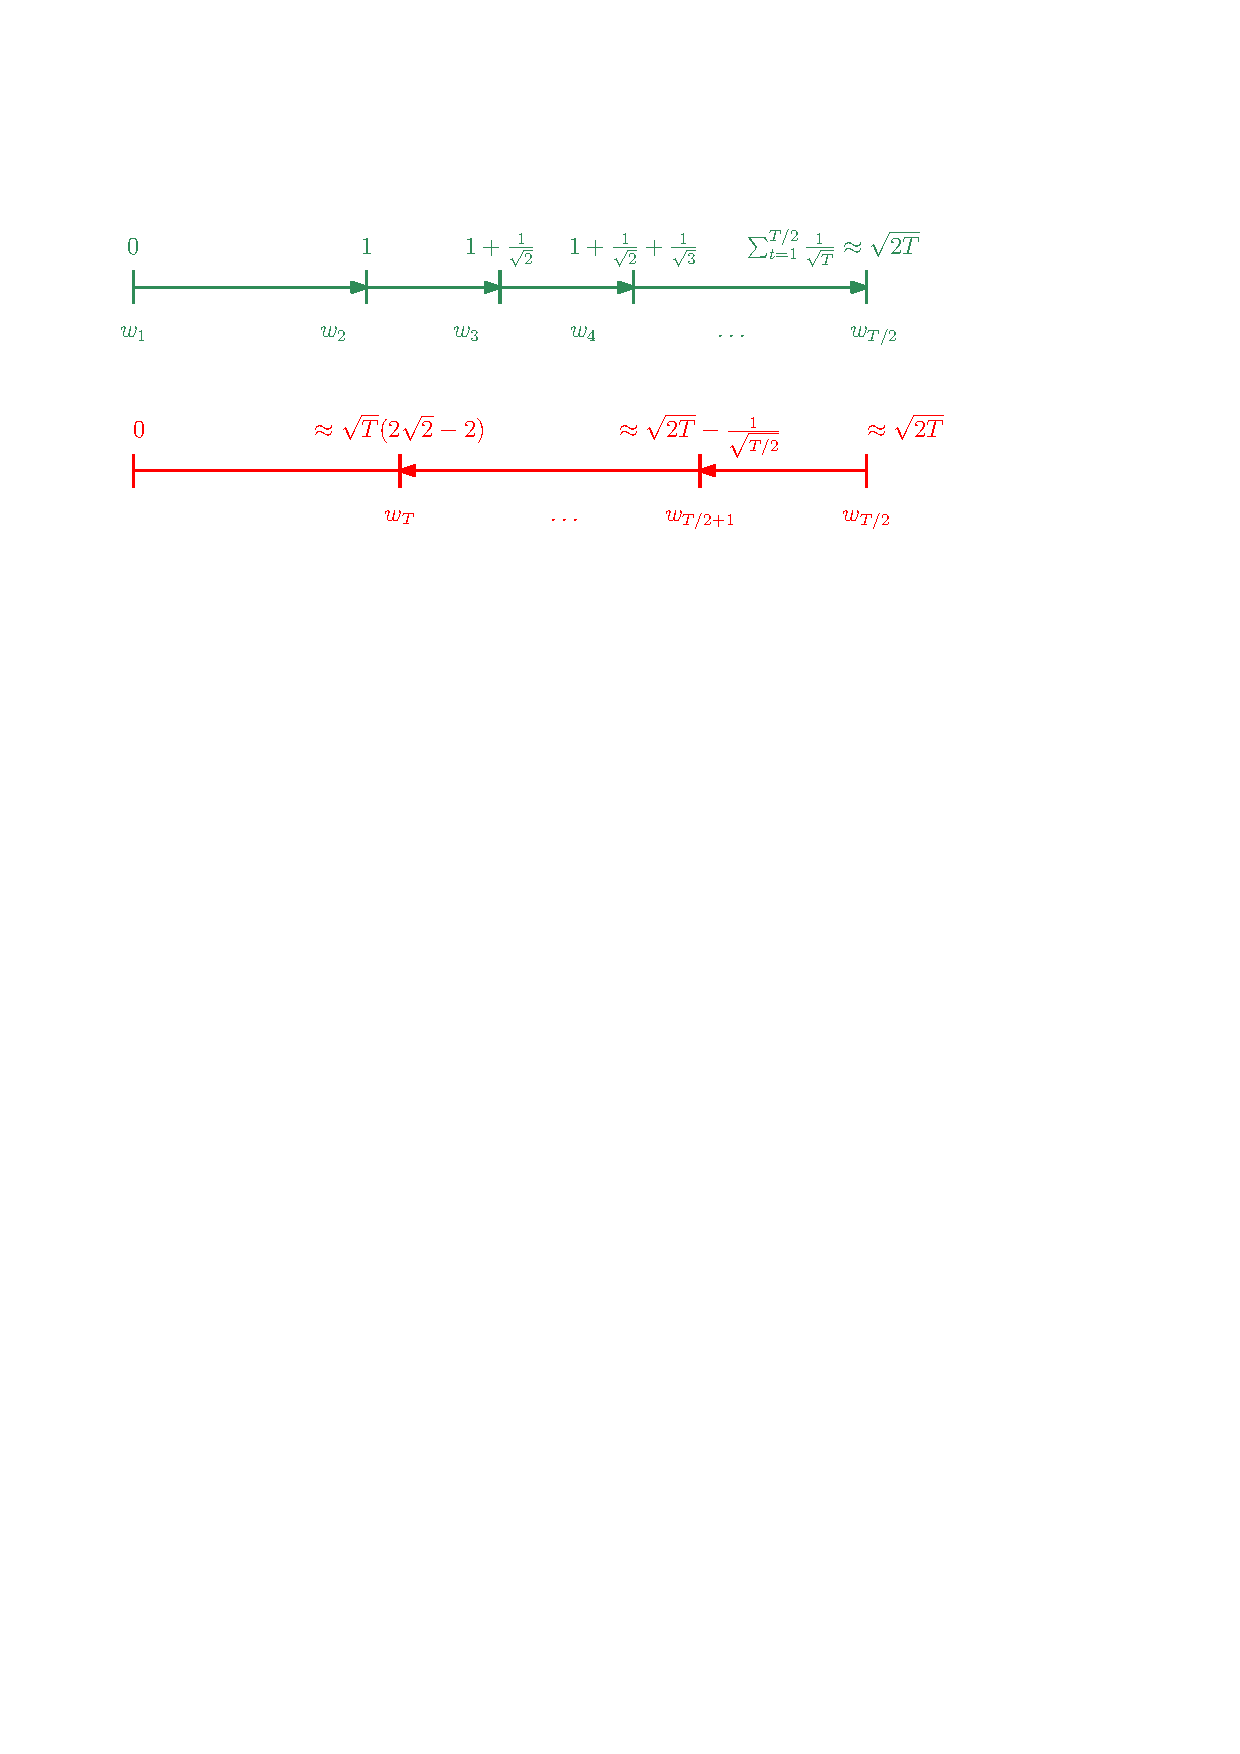
\includegraphics[scale=0.5]{gd-lower-bound}
\end{center}

$$
\Regret_T(0) = \sum_{t=1}^T w_t \ell_t = \textcolor{ForestGreen}{-\sum_{t=1}^{T/2} w_t} \quad \textcolor{Red}{+ \sum_{t={T/2+1}}^T w_t} \ge \frac{T^{3/2}}{20}
$$
\end{frame}

%%%%%%%%%%%%%%%%%%%%%%%%%%%%%%%%%%%%%%%%%%%%%%%%%%%%%%%%%%%%%%%%%%%%%%%%%%%%%%%%%%%%%%%%%%
\begin{frame}
\frametitle{FTRL to the Rescue}

Gradient Descent:
$$
w_t = - \sum_{s=1}^{t-1} \eta_s \ell_s
$$
FTRL:
$$
w_t = - \eta_t \sum_{s=1}^{t-1} \ell_s
$$

\begin{theorem}[Orabona-P. '15]
FTRL with $\eta_t = \frac{1}{\sqrt{\sum_{t=1}^T \norm{\ell_t}_2^2}}$
satisfies for all $u \in \R^N$,
$$
\Regret_T(u) \le \left(\frac{\norm{u}_2^2}{2} + 2.75 \right) \sqrt{\sum_{t=1}^T \norm{\ell_t}_2^2} \ + \ 3.5 \sqrt{T} \max_{t \le T} \norm{\ell_t}_2
$$
\end{theorem}

\end{frame}


\end{document}
